\documentclass{sig-alternate-05-2015}


\usepackage{cite}
\usepackage{url}
\usepackage{color}
\usepackage{tikz}
\usepackage{balance}
\usepackage{caption}
\usepackage{soul} % Used for highlighting % \hl{this is some highlighted text}
\usepackage{times} % Used for formatting formatting url footnotes
\urlstyle{same} % Used for formatting formatting url footnotes
\usepackage[binary-units=true]{siunitx}
\usepackage[caption=false]{subfig}
\usepackage{multicol}
\usepackage{flushend} %% Helps to balance out the last columns

\setlength\floatsep{1.25\baselineskip plus 3pt minus 2pt}
\setlength\textfloatsep{0.7\baselineskip plus 3pt minus 2pt}
\setlength\intextsep{1.15\baselineskip plus 3pt minus 2 pt}

\newcommand{\todo}[1]{\textcolor{cyan}{\textbf{[#1]}}}
\newcommand{\sam}[1]{\textcolor{green}{{\it [Sam says: #1]}}}
\newcommand{\dan}[1]{\textcolor{blue}{{\it [Dan says: #1]}}}
\newcommand{\nuthan}[1]{\textcolor{red}{{\it [Nuthan says: #1]}}}


% Define flow chart styles
\tikzstyle{decision} = [diamond, draw, fill=blue!20,
    text width=15em, text badly centered, node distance=3cm, inner sep=0pt]
\tikzstyle{block} = [rectangle, draw, fill=blue!20,
    text width=15em, text centered, rounded corners, minimum height=4em]
\tikzstyle{line} = [draw, -latex']

\usetikzlibrary{shapes,arrows, positioning} % Needed for analysis diagram







\begin{document}
\toappear{}

\title{Darwin: A Static Analysis Dataset of Malicious and Benign Android Apps}


\author{
\alignauthor
Nuthan Munaiah, Casey Klimkowsky, Shannon McRae, Adam Blaine,  Samuel~A.~Malachowsky, Cesar Perez, and Daniel E. Krutz \\
       \affaddr{Rochester Institute of Technology, Rochester, NY, USA}\\
       \email{\{nm6061, cek3403, smt9020, amb8805, samvse, cap7879, dxkvse\}@rit.edu}
       \alignauthor
} % Must not be a space above this

\maketitle 
\begin{abstract} %%% See overleaf
\hl{OLD VERSION} 
The Android platform comprises the vast majority of the mobile market. Unfortunately, Android apps are not immune to the issues that plague conventional software including security vulnerabilities, bugs, and permission based problems. In order to address these issues, we need a better understanding of the apps we use everyday. Over the course of more than a year, we collected and reverse engineered 64,868 Android apps from the Google Play store as well as 1,669 malware samples collected from several sources. Each app was analyzed using several static analysis tools to record a variety of quality and security related information about each of them. This dataset contains apps from 41 different categories, and a total of 576,174 permissions, 39,780 unique signing keys and 125,159 over-permissions. We present our data in an easy to use, publicly available website along with a database which researchers may downloaded for future evaluations. The data set and a brief set of analytics are presented on our website: http://darwin.rit.edu

\end{abstract}


\begin{CCSXML}
<ccs2012>
<concept>
<concept_id>10003120.10003138.10003139.10010905</concept_id>
<concept_desc>Human-centered computing~Mobile computing</concept_desc>
<concept_significance>300</concept_significance>
</concept>
</ccs2012>
\end{CCSXML}

\ccsdesc[300]{Human-centered computing~Mobile computing}
\printccsdesc

\keywords{Mobile Computing, Software Quality, Mobile Security}

\section{Introduction}

Unfortunately, Android applications (apps) frequently suffer from the same problems which also plague conventional software: security vulnerabilities, defects, adherence to coding standards, and numerous other issues. Additionally, malicious developers create malware for the purpose of exploiting users or devices for profit. There are innumerable areas of Android research which examine both malicious and benign apps in a variety of quality, security, and evolutionary perspectives. Unfortunately, collecting this information is frequently a time consuming or difficult task. In order to assist researchers examining Android apps for a variety of security and quality perspectives, we have created a substantial statistical dataset for them to use in their own studies. Our goal was to create an information set which could be used in a wide variety of mobile research including security, quality and evolution analysis. Our dataset contains information about 64,868 reverse engineered apps from Google Play and 1,669 apps collected from known malware sources.

In this paper we discuss (i) the data collection and analysis process, (ii) an easy to use web application to share project information and provide access to raw data in our .sqlite database, and (iii) lay the groundwork for future research by exploring a variety of vital areas of future research. Due to usage agreements, we were unable to publicly share all examined Android app (apk) files. If any researchers wold like access to this dataset, they should contact the authors of the paper.


\section{Related Work}
\label{sec: relatedworks}

There have been many studies which analyzed mobile apps on a large scale. Sarma~\emph{et al.}\cite{Sarma:2012:APP:2295136.2295141} evaluated several large datasets, including one with 158,062 Android apps to gauge the risk of installing the app, with some of the results broken down by category. However, this work did not analyze the apps using the range of static analysis tools presented in this paper. Viennot~\emph{et al.}\cite{Viennot:2014:MSG:2637364.2592003} developed a tool called `PlayDrone' which they used to examine the source code of over 1,100,000 free Android apps. Unfortunately, they largely only used existing information which could be gathered from Google Play and only examined features such as library usage and duplicated code. They did not study areas such as quality, security vulnerability levels, and over-permissions, which were a part of our analysis. Felt~\emph{et al.} described some common developer errors found using their tool Stowaway, including confusing permission names, the use of depreciated permissions, and errors due to copying and pasting existing code~\cite{Felt:2011:APD:2046707.2046779}. Krutz~et al.\cite{krutz2015FDroid} created a public dataset of over 1,100 Android apps from the F-Droid\footnote{\url{https://f-droid.org/}} repository and analyzed a much smaller number of apps than our study and focused more on the lifecycle of the apps and how each iteration of the app evolved with every version control commit.

There are several other websites which gather metrics about Android apps. AppAnnie\footnote{\url{https://www.appannie.com}} and Koodous\footnote{\url{https://koodous.com/}}, collect Android apps and perform several types of analysis on each of them including downloads of the app over time and advertising analytics. However, no known services perform the same types of static analysis and comparisons on apps that we do. VirusTotal\footnote{\url{ https://www.virustotal.com/}} is a service which is able to analyze files and URLs for viruses. Darwin does not analyze Android apps to determine if they are viruses, it checks for vulnerabilities in apps whose assumed intention is to be non-malicious. Several works have created malware repositories containing malicious application (apk) files for download, including the Contagio Mobile Mini Dump\footnote{\url{http://contagiominidump.blogspot.com}} and the Malware Genome Project\footnote{\url{http://www.malgenomeproject.org/}}.


%\vspace{4 mm}
\section{Dataset Construction}
\label{sec: datasetconstruction}

%%~\cite{Martin:2015:ASP:2820518.2820535} %%% App sampling problem

% An overview of the process is shown in Figure~\ref{fig:analysisprocess}. %% Removed based on feedback

Our dataset was built by collecting apps and analyzing them using several well-known security and quality static analysis tools. Our paramount process concern was accuracy; problems with even a very small percentage the apps or at any stage in the collection or reverse engineering process could have had devastating results in the accuracy of our work. To achieve an appropriate level of quality, we relied upon unit testing, manual verification, and frequent test runs. Because of this, the optimization and testing phases took the largest share of development time for the project.

%%% Look at the reviews for different quality steps that I need to mention. Add in if there is room for this in the future.



% An overview of the process is shown in Figure~\ref{fig:analysisprocess}. %% Removed based on feedback
%\begin{figure}[]
%\begin{center}
%
%% Define block styles
%\tikzstyle{line} = [draw, -latex']
%
%%\tikzstyle{cloud} = [draw, ellipse,fill=white!20, node distance=1.5cm, minimum height=2em]
%\tikzstyle{cloud} = [draw=none, ellipse,fill=white!20, node distance=1.5cm, minimum height=2em]
%
%\tikzstyle{block} = [rectangle, draw, fill=white!20, text width=5em, text centered, rounded corners, minimum height=4em]
%\tikzstyle{c} = [draw, cylinder, shape border rotate=90, aspect=0.75, minimum height=70, minimum width=30]
%
%\begin{tikzpicture}[node distance = 1.1cm, auto]
%
%    % Place nodes
%     \node [cloud] (init) {APK Collection};
%     \node [block, below of=init] (ApkFiles) {ApkFiles};
%     \node [cloud, below of=ApkFiles] (Decompile) {Decompile};
%     \node [block, below of=Decompile] (DecompiledFiles) {Decompiled Files};
%     \node [cloud, below of=DecompiledFiles] (JavaAnalysis) {Java Analysis};
%    % \node [cloud, right of=ApkFiles] (apkanalysis) {Stowaway AndroRisk};
%    % \node [c, right of=DecompiledFiles] (SqliteDB) {SqliteDB};
%     \node[c] (SqliteDB) [below right=-1.0cm and 2.4cm of DecompiledFiles]{SQLiteDB};
%
%    \node[cloud] (apkanalysis) [below right=-0.9cm and 2.0cm of ApkFiles]
%       {APK Analysis};
%
%    % Draw edges
%    \path [line] (init) -- (ApkFiles);
%    \path [line] (ApkFiles) -- (Decompile);
%    \path [line] (Decompile) -- (DecompiledFiles);
%    \path [line] (DecompiledFiles) -- (JavaAnalysis);
%    \path [line] (ApkFiles) -- (apkanalysis);
%    \path [line] (apkanalysis) -- (SqliteDB);
%    \path [line] (JavaAnalysis) -- (SqliteDB);
%    \path [line] (Decompile) -- (SqliteDB);
%
%\end{tikzpicture}
%\caption{Analysis Process}
%\label{fig:analysisprocess}
%\end{center}
%\end{figure}


\label{sec: collection}
\subsection{Step 1: Collect APK files}

Our initial step was to collect app meta data information and APK files from Google Play. We constructed a custom-built data collection system, which uses ~\emph{Scrapy}\footnote{http://scrapy.org} as a foundation. Our goal was to collect a diverse set of apps, so apps were randomly selected and collected by Scrapy from Google Play and did not target specific apps, or specific versions of apps. Our data collect process took place over the course of more than a year.

Malware samples were collected from the Contagio Mobile Mini Dump and the Malware Genome Project. The Contagio Mobile Mini Dump has been collecting malware affecting many platforms, including Android, for several years. In this study, 160 malware examples from the Contagio Mobile mini dump were used. The Malware Genome Project began in 2010 and has collected a substantial number of mobile malware. For our analysis, we used 1,257 examples from 49 malware families.


\subsection{Static Analysis}


%%%% Feedback: Explain the reverse engineering process a bit more

Our first step was to reverse engineer our collected apps using a previously established process~\cite{Lee_2013}. The app was
was first unzipped using a simple unix command and then two open source tools were used to complete the reverse engineering process:
\begin{itemize}
    \setlength{\itemsep}{0pt} %Cut down on spacing for the different items in the list
    \setlength{\parskip}{0pt} %Cut down on spacing for the different items in the list
    \setlength{\parsep}{0pt}  %Cut down on spacing for the different items in the list

  \item \textbf{dex2jar\footnote{\url{https://code.google.com/p/dex2jar/}}:} Convert the .dex file into a .jar file. A java jar command is then used to convert this to .class files.
  \item \textbf{jd-cmd\footnote{\url{https://github.com/kwart/jd-cmd}}:} Converts .class files to .java.
\end{itemize}

The de-compilation process is shown in Figure~\ref{fig:extractionprocess}.

% ~\cite{Lee_2013} %% This diagram is largely copied from here

% Define block styles
\tikzstyle{line} = [draw, -latex']
\tikzstyle{cloud} = [draw, ellipse,fill=white!20, node distance=2.2cm,
    minimum height=2em]

	\begin{figure}[h]
	\begin{center}

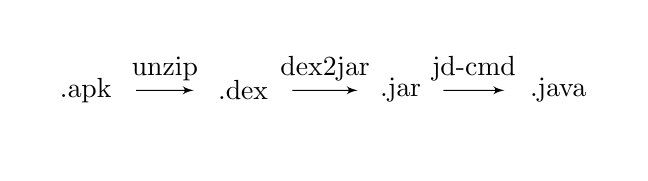
\begin{tikzpicture}[node distance = 2cm, auto]
    % Place nodes
     \node [cloud] (init) {.apk};
     \node [cloud, right of=init] (dex) {.dex};
     \node [cloud, right of=dex] (jar) {.jar};
     \node [cloud, right of=jar] (java) {.java};

     \path [line] (init) -- node {unzip}(dex);
     \path [line] (dex) -- node {dex2jar}(jar);
     \path [line] (jar) -- node {jd-cmd}(java);

\end{tikzpicture}
\caption{APK Extraction Process}
\label{fig:extractionprocess}
\end{center}
\end{figure}


We next used several existing static analysis tools to analyze the apps for a variety of security and quality metrics.

\textbf{Stowaway\cite{Felt:2011:APD:2046707.2046779}:} The~\emph{principle of least privilege} states that each app should request the minimum number of permissions that it needs to function. Requesting more permissions than required creates unnecessary security vulnerabilities~\cite{saltzer1975protection}. Android operates under a permissions-based system where apps must be granted specific functionality before they may be used. Some of these include access to the camera, contacts, microphone, and location data.

Over-permissions are considered security risks, and under permissions are considered quality risks. The primary difference between requested permissions and over-permissions is the consideration of whether the app actually needs them or not. Under and over permissions of an app, reported by Stowaway, were recorded in our data. Modifications were made to the existing version of Stowaway to accommodate our process and stay current with updated Android permissions.


\textbf{AndroRisk\footnote{\url{https://code.google.com/p/androguard}}:}AndroRisk reports the risk indicator of an application concerning potential malware and determines the security risk level of an application by examining several criteria. Some of these criteria include the presence of permissions which are deemed to be more dangerous (i.e. access to the internet, SMS messages, or payment systems) and the presence of generally more dangerous functionality in the app (i.e. a shared library, use of cryptographic functions, the reflection API). We recorded the reported risk level for each APK file.


 \textbf{CheckStyle\footnote{\url{http://checkstyle.sourceforge.net}}:} This tool measures how well developers adhere to coding standards such as annotation usage, size violations, and empty block checks. We recorded the total number of violations of these standards. Default application settings for Android were used in our analysis. While adherence to coding standards may seem to be a trite thing to measure, compliance to coding standards in software development can enhance team communication, reduce program errors, and improve code quality~\cite{Li:2005:ETC:1095714.1095770}.

 \textbf{Jlint\footnote{\url{http://jlint.sourceforge.net}}:} This examines Java code to find bugs, inconsistencies, and synchronization problems by conducting a data flow analysis and building lock graphs. We recorded the total number of discovered bugs per app. This tool was selected over FindBugs\footnote{\url{http://findbugs.sourceforge.net}} for its ability  to analyze the applications much faster while providing accurate results~\cite{rutar2004comparison}.

 \textbf{APKParser\footnote{\url{https://github.com/joakime/android-apk-parser}}:} A tool designed to read various information from Android APK files including the version, intents, and permissions. We used the output from this tool to determine the application version, minimum SDK, and target SDK.
A dataset of open-source Android applications

\textbf{Keytool:\footnote{\url{https://docs.oracle.com/ javase/6/docs/technotes/tools/windows/keytool.html}}} A key and certificate management utility which we use to determine various signing information including owner and issuer information and the MD5, Sha1, and Sha256 signing keys.

We also recorded other metrics about each application including total lines of code, number of Java files, application version, target SDK, and minimum SDK. Stowaway and AndroRisk were able to analyze the raw APK files, while CheckStyle, Jlint, and Nicad required the APK files to be decompiled. All results were recorded in an SQLite database, which is publicly available on the project website.


%%%% Added this section
\subsection{Challenges}

There were several significant challenges which had to be overcome in our collection and analysis process. Although using Scrapy was an immensely beneficial, collecting such a large number of apk files for over a year was not a trivial process. There were several cases where our collection tool needed to be modified due to alterations with Google Play. These required changes would occur intermittently and would often disrupt our collection process.

One of the largest challenges we needed to overcome was analysis time. Although we worked very hard to make the analysis process as fast as possible, the reverse engineering and analysis process for an app took from 2 to 10 minutes to complete. This meant that we were limited in the amount of apps that we could analyze on a daily basis. Frustratingly, for an unknown reason we were unable to reverse engineer a small number (less than .5\%) of collected apps. Our hypothesis is that a library or obfuscated portion of code created problems for our analysis, but unfortunately we were unable to determine a root cause for the problem.




%Two examples include alterations made to Google Play which affected our year(+) long collection process and making our reverse engineering and analysis process efficient enough to handle such a large quantity of apps.

\section{Analytics \& Data Sharing}
\label{sec: Website}

We have shared all of our project results on our project website: \textbf{\url{http://darwin.rit.edu}}. Our goal is to provide a robust, and easy to use mechanism for other researchers and interested parties. Android users may search for particular apps on the website to view a variety of quality and security related metrics (as well as comparing different versions). A researcher may utilize the more advanced features of the website and download the entire dataset for their own analysis.

All data is available in three sqlite databases--- one for Google Play and one for each of the two malware sources. A database schema is provided on the project website to assist others in understanding our data set. Unfortunately we could not make the .apk files collected from Google Play available due to both size restrictions (the total collected apk files exceeded $\SI{680}{\giga\byte}$) and possible copyright infringement. We could not make the malware available due to usage agreements.



\subsection{Exploring the Dataset}

%We have created several examples to demonstrate both the breadth and depth of our dataset; t

Table \ref{Table:overallStats} provides an overview of some high level statistics including the total number of categories, unique signing keys, total permissions, total under-permissions, and total over-permissions. The complete dataset and robust instructions may be found on the project website.


\begin{table}[ht]
\begin{center}
\caption{Overview of Collected Data}
\label{Table:overallStats}
 \begin{tabular}{ | l | c | c |} \hline

	 \bfseries Total & \bfseries   Google Play & \bfseries Malware \\ \hline
	
    %Max Versions\todo{rename?} &	12 \\ \hline
	Unique Category & 41 & n/a \\ \hline
	Apps &	64,868 & 1,669 \\ \hline
	Unique Signing Keys  & 39,592 & 188 \\ \hline

	Requested Permissions &	558,216 & 17,958 \\ \hline
	Intents &	232,645 & 3,331 \\ \hline
	Over-Permissions   & 125,159 & 7,288 \\ \hline
	Under-Permissions  & 228,475 & 2,222 \\ \hline
	
	%Unique Apps &	X \\ \hline
	%Apps with multiple versions &	X \\ \hline
%	X &	X \\ \hline
	
        	 	
  \end{tabular}
\end{center}
\end{table}


While our primary goal was not to target specific versions of apps, we did collect numerous versions of the same app. Table~\ref{Table:versionCounts} displays the number of analyzed apps and their version counts. Analyzing multiple app versions can be extremely useful for a variety of research activities including quality and security perspectives.

\begin{table}[ht]
\begin{center}
\caption{Collected App Version Counts}
\label{Table:versionCounts}
 \begin{tabular}{ | l | c | } \hline

	  \bfseries Collected Versions & \bfseries   Count \\ \hline
	
	2+ &	6,546 \\ \hline
	3+ &	1,853 \\ \hline
	4+ &	823 \\ \hline
	5+ &	421 \\ \hline
    10+ & 41 \\ \hline
        	 	
  \end{tabular}
\end{center}
\end{table}


Using a custom built analysis tool, we collected each app's requested permissions from the reverse engineered~\emph{AndroidManifest.xml} file. Table~\ref{Table:permissionCounts} displays the five most requested permissions from Google Play apps, along with the number collected from malware.

\begin{table}[ht]
\begin{center}
\caption{Top Permission Counts}
\label{Table:permissionCounts}
 \begin{tabular}{ | l | c | c | } \hline

	  \bfseries Permission & \bfseries   Google Play & \bfseries Malware \\ \hline
	
	INTERNET &	73,484 & 943  \\ \hline
	ACCESS\_NETWORK\_STATE &	62,494 & 821 \\ \hline
	WRITE\_EXTERNAL\_STORAGE &	43,904 & 618\\ \hline
	READ\_PHONE\_STATE &	31,345 & 890 \\ \hline
	WAKE\_LOCK & 26,144 & 316 \\ \hline	
        	 	
  \end{tabular}
\end{center}
\end{table}


We collected the number of apps signed using the same developer key for both the Google Play and malware apps. These values are shown in Table~\ref{Table:md5Counts}. A signing key is used to verify the origin of the app; only the developer holds the proper key used to sign a created app.

\begin{table}[ht]
\begin{center}
\caption{Apps Signed Using Same MD5 Key}
\label{Table:md5Counts}
 \begin{tabular}{ | l | c | c | } \hline

	  \bfseries App Count & \bfseries   Google Play & \bfseries Malware \\ \hline



	
	10+ &	12,981	& 576 \\ \hline	
%	15	& 10,377	& 424 \\ \hline	
%	20	& 8,794	& 360 \\ \hline	
	25+	& 7,703	& 269 \\ \hline	
%	30	& 7,059	 & 214 \\ \hline	
%	35	& 6,577	& 150 \\ \hline	
%	40	& 6,211	& 111 \\ \hline	
	50+	& 5,608	& 66 \\ \hline	
	100+ &	3,992	  & - \\ \hline	
%	150&	3,527	 & - \\ \hline	
%	200&	3,152	 & - \\ \hline	
	250+&	2,916	 & - \\ \hline	
%	300&	2629	 & - \\ \hline	
%	350&	2629	 & - \\ \hline	
%	400&	2629	 & - \\ \hline	
	500+&	2,629	 & - \\ \hline	
	
	
	
        	 	
  \end{tabular}
\end{center}
\end{table}









\subsection{Analytical Results}

The project website contains pre-built reports and information pages which may be used to view aggregate or individual app data. This includes some pre-built reports in .csv format, some of which include: all reported over-permissions for each app, requested permissions for each app, and all reported static analysis metrics. The site also contains several pre-built graphical representations of the data. %An example graph showing the rate of over-permissions found in each category is shown in Figure~\ref{fig:overPrivsGenre}.


%%% Removed for space reasons
%%%% Check to make sure this image looks ok in the print out
% \begin{figure}[h]
%\centering
%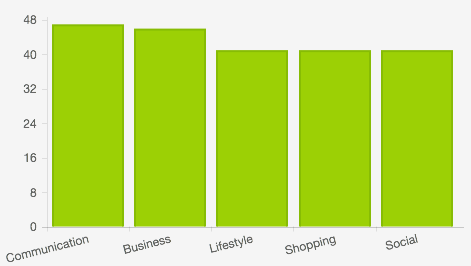
\includegraphics[width=\columnwidth, angle = 0]{images/OverPrivsGenre.png}
%\caption{Rates of Over-permissions by Category}
%\label{fig:overPrivsGenre}
%\end{figure}


\begin{figure}[h]
\centering
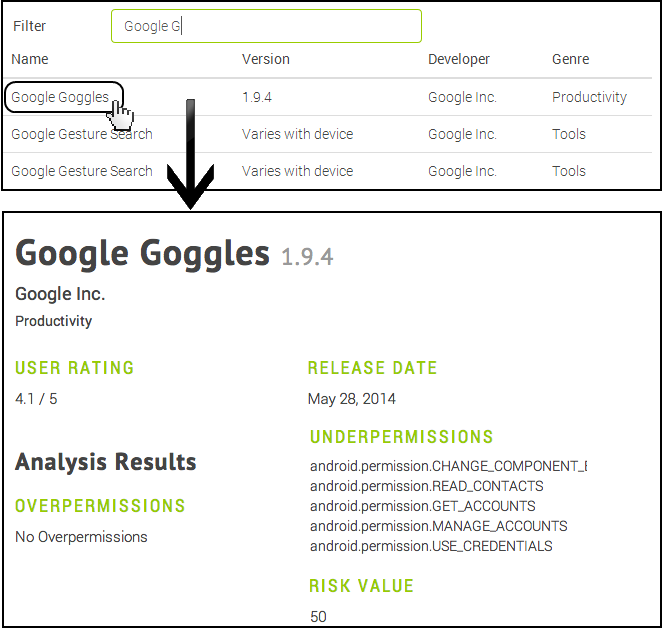
\includegraphics[scale=0.4]{images/Google_Googles_ICSE.png}
\caption{Example App Search}
\label{fig:appSearch_all}
\end{figure}




Users may explore our data set in two primary ways. Users may search for the results of individual apps as shown in Figure~\ref{fig:appSearch_all}, or they may explore the data by writing their own queries against the dataset right on the webpage as shown in Figure~\ref{fig:webpagequery}. Users may also choose to download our entire raw data set, which is in sqlite format.
%



% Prebuilt .csv reports
%









\begin{figure}[ht!]
\centering
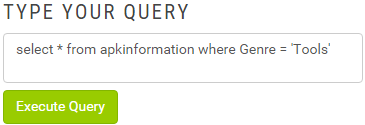
\includegraphics[width=\columnwidth, angle = 0, scale=.8]{images/webpageQuery2.png}
\caption{Webpage Search Query}
\label{fig:webpagequery}
\end{figure}






\subsection{Enabled Research}


% Provide Introduction
This dataset provides a wide range of benefits for Android users, researchers, and app developers and we will next provide several usage scenarios for our provided data.

\textbf{Facilitate research on Google Play apps.} A goal of our work is to allow others to extend upon our research. Since we collected a variety of information from Google Play and from static analysis tools, comparisons could be done against the user ratings of the apps from a variety of quality and security-related metrics. Permissions data (558,216 total collected permissions) could be used to provide insight in numerous areas including the tendencies of permissions use and the popularity of various permissions.

We collected several forms of signing information about each app which could also prove useful for future researchers. Collecting and validating previous app versions is difficult, and while we are unable to provide the actual .apk file, we are able to provide the signing key --- which may be used to verify the authenticity of other apps. Although developers often use different app and developer names, one way to identify the creator of an app is through the md5 key. Individual developers may use the same md5 value to sign multiple apps, which is a reliable method of identifying the actual creator of an app. Additionally, we collected  other signing information about the apps including various owner and issuer values and the sha1 and sha256 values.

\textbf{Facilitate research on Malware.}
To better detect and defend against malware, we need to understand more about it such as how it is created, evolves, and its common characteristics. Including data from benign and malicious apps will enable researchers to study these apps in a variety of ways including how malware is evolving, signing information, app quality, and requested permissions.





\section{Limitations \& Future Work}
\label{sec: Limitations}

There are several limitations to our data set and possible improvements. We only examined free apps, thus excluding a significant population (paid apps) in our analysis. Although our reverse engineering process has been demonstrated to be highly effective in previous research~\cite{chawla2014transfiguring}, all such processes contain possible flaws which could lead to imperfections in the analysis process. We used Stowaway to analyze apps for permission misuse, however new tools such as PScout~\cite{au2012pscout} could have been used to conduct this analysis.

Along with the rating of an app, user reviews are an effective way of measuring a user's perception of an app~\cite{khalid2015examining}. Future work may be done to collect the associated user reviews and include these results in the data set as well. Our goal was to collect a wide variety of apps and did not target specific apps for collection. Future work may be done to target specific apps to ensure that numerous versions of each app are collected. We did not target specific apps or versions for this study since our goal was to collect a diverse set of apps as possible. Analyzing numerous versions of the same app can provide valuable insight into the evolution of the app from a security, and quality perspective.


\section{Conclusion}
\label{sec: conclusion}

We created a valuable, publicly accessible dataset by collecting and analyzing 64,868 apps from Google Play and various malware sources. This dataset is beneficial to developers, researchers, and Android users in not only understanding existing apps, but in how apps are developed, evolve, and are maintained. The collected data is publicly available on the project website: \url{http://darwin.rit.edu}

\balance
\bibliographystyle{abbrv}
\bibliography{DarwinData}

% That's all folks!
\end{document}


% ************************


% Schema: https://www.draw.io/?state=%7B%22folderId%22:%220B2pV6O4YmViscWlLd1pmak1Ba28%22,%22action%22:%22create%22,%22userId%22:%22105339315238212488590%22%7D#G0B2pV6O4YmVisZHFhR2hJOTVGdVk



%%% Todo
%	Provide schema of dataset on the Darwin webpage




% Notes:
%	"Google Play" - it is 2 words




% Submission:
%	




